%% Hello emacs, this is -*- latex -*-
\typeout{ ====================================================================}
\typeout{ This is file futuro.tex, created at 13-Jun-2004 }
\typeout{ Maintained by Andre Rabello dos Anjos <Andre.dos.Anjos@cern.ch> }
\typeout{ ====================================================================}

\chapter{Conclusões e Trabalhos Futuros}
\label{chap:future}

Como foi visto, o LVL2 é o primeiro nível do sistema de classificação do ATLAS
que analisará o evento tendo em vista suas características globais. Para cada
objeto (RoI) destacado no LVL1, o LVL2 executará rotinas de classificação,
visando confirmar os objetos identificados pelo nível antecessor e, assim,
discriminar o evento. Dentre os objetos importantes para o experimento ATLAS,
encontram-se os elétrons, representando uma boa parcela dos objetos que serão
analisados pelo LVL2. Elétrons, por sua vez, são comumente contaminados por
jatos, quando esses interagem de forma similar com os calorímetros. Portanto,
um classificador elétron/jato mais eficiente é vital no LVL2.

O classificador elétron/jato tem o objetivo de discriminar jatos e elétrons,
preservando o máximo de elétrons que for possível, já que estas partículas são
portadoras da informação que se deseja detetar no ATLAS: o bóson de
Higgs. Elétrons e jatos são comumente distinguidos pela forma que depositam
energia nos calorímetros do ATLAS. Jatos, por serem um conglomerado de
partículas hadrônicas, usualmente penetram com mais profundidade nos
calorímetros, também produzindo uma cascata mais espalhada, enquanto elétrons
produzem cascatas menores e mais colimadas (Figuras~\ref{fig:eroi},
\ref{fig:jroi} e \ref{fig:ejet}).

\section{Análise do cenário atual}

Métodos clássicos de deteção aproveitam-se das características físicas da
deposição de energia nos calorímetros para obter uma alta eficiência de
classificação (95\% para elétrons e 88,4\% para jatos, como visto na
Seção~\ref{sec:bi-results}), extraindo quatro variáveis físicas com alto poder
de discriminação. Os métodos clássicos, no entanto, desconsideram jatos que
possuem um padrão de decaimento extremamente semelhante ao de elétrons e se
diferenciam apenas por sutilezas no seu processo de interação com os
calorímetros do ATLAS. Para classificar corretamente estes eventos, um sistema
tão simplificado não pode ser empregado.

\subsection{Somas em anel}

Embora não seja uma solução que se aproveite da máxima granularidade dos
calorímetros do ATLAS, a discriminação usando as quatro variáveis clássicas
compacta o vetor de entrada de cerca de 1.000 células para 4 quantidades,
mantendo um desempenho satisfatório. Re-avaliando o espaço de entrada inicial
(as 1.000 células) e observando-se a física de decaimento dos objetos de
interesse, no entanto, é possível elaborar um sistema também compacto, mas que
preserve melhor as diferenças nos padrões de interação calorimétrica entre as
duas classes de partículas. Nesse novo sistema, identifica-se o pico de
deposição energética em cada camada e executa-se um procedimento de soma em
anéis concêntricos (Seção~\ref{sec:aneis}), formando-se um total de 58 novas
variáveis, que representam o objeto de maneira mais atraente para um
classificador.

Projetando-se, então, um classificador neural para este novo espaço de
entrada (de dimensão 58), é possível obter uma eficiência de classificação
bastante acima do que foi obtido usando-se as quatro variáveis discutidas. A
figura~\ref{fig:test17} mostra a curva característica do Teste 17 da
Tabela~\ref{tab:ring-neural}, quando comparada ao melhor discriminador neural
utilizando as quatro variáveis clássicas e ao discriminador linear, também para
variáveis clássicas. Como é possível ver nessa figura, a eficiência de
classificação usando anéis é bastante superior àquelas usando as quantidades
clássicas.

\begin{figure}
\begin{center}
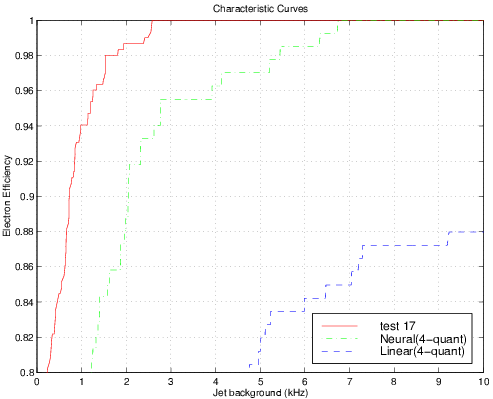
\includegraphics[scale=0.65]{msc/efficiency-17}
\end{center}
\caption{Eficiência comparativa entre o melhor discriminador usando 58 anéis e
aqueles baseados nas quatro quantidades físicas.}
\label{fig:test17}
\end{figure}

\subsection{Relevância}

O espa\-ço gerado a partir das 58 somas em anel pode ainda ser reduzido,
observando-se a rele\-vân\-cia (Se\-ção~\ref{sec:relevance}) de cada uma das
entradas para o classificador neural proposto. A relevância, como foi visto,
mede o impacto na classificação, quando se substitui uma das variáveis de
entrada pela estimativa de sua média estatística.

Aplicando-se o estudo de rele\-vân\-cia, tanto aos classificadores baseados nas
vari\-á\-veis clás\-sicas quanto aqueles baseados nas somas em a\-néis, é
pos\-sí\-vel ver que nem todas as vari\-á\-veis dispo\-ní\-veis para a
classifica\-ção são, de fato, relevantes para o discriminador neural. Para o
caso das variáveis clássicas, a remoção da variável \eratio\ e o treinamento de
um novo classificador (agora baseado em um novo espaço tri-dimensional) não
demonstra um impacto profundo no poder de classificação de elétrons e jatos,
como é possível notar na Figura~\ref{fig:class-relev-best}.

No classificador baseado nas somas em anel, a redução da dimensão do espaço de
entrada, de 58 para 20 (eliminando 38 anéis!) também não influencia de forma
significativa (Figura~\ref{fig:eff-cut1}) a discriminação elétron/jato. Algum
impacto, no entanto, pode ser observado continuando-se a reduzir a
dimensionalidade do espaço de entrada. Ainda assim, classificadores com apenas
5 dos 58 anéis mantiveram desempenho acima do melhor desempenho que foi obtido
com as 4 variáveis clássicas usando um discriminador neural
(Figura~\ref{fig:last-effic}). Estes resultados indicam que há melhores
maneiras de compactar os dados de uma RoI, de forma a discriminar mais
eficientemente elétrons e jatos.

O excelente desempenho dos discriminadores baseados nas somas em anel advém do
aproveitamento da máxima granularidade do detetor, sem que as sutilezas nos
padrões de decaimento dos objetos sejam perdidas, o que não é possível observar
quando aplica-se o estudo com as variáveis clássicas. Esta compactação em
anéis, ademais, permite um estudo mais detalhado da relevância das diversas
camadas dos calorímetros do ATLAS, quando expostas ao problema da discriminação
de objetos e.m.. Através deste estudo, é possível estabelecer critérios de
simplificação (cortes de dimensionalidade) do discriminador de forma a torná-lo
suficientemente rápido, mas ainda mantendo uma eficiência de discriminação
acima das possíveis soluções com o sub-espaço de variáveis clássicas, como foi
possível observar na Figura~\ref{fig:last-effic}.

A \textbf{não} utilização dos dados da terceira camada e.m. dos calorímetros
não impediu que uma eficiência maior fosse atingida, utilizando a soma em
anéis. Possivelmente, a inclusão dos dados desta camada em estudos posteriores
possa mostrar uma melhora significativa no método proposto, acentuando ainda
mais as diferenças entre o método de discriminação hoje empregado no segundo
nível de filtragem do ATLAS e aquele desenvolvido neste trabalho.

\section{Potencial para o Futuro}

Os trabalhos apresentados neste texto indicam que a compactação excessiva de
informação no LVL2 poderá comprometer o poder de classificação global do
Sistema de Filtragem do ATLAS. A redução da dimensionalidade de entrada, dos
cerca de 1.000 canais iniciais para apenas 4 quantidades discriminantes
introduz ineficiências que penalizam o desempenho do LVL2. A utilização de uma
compactação que observe a quantidade de informação em cada canal é, portanto,
intuitivamente ótima, já que maximizará o potencial de deteção do sistema.

Para confirmar esta previsão na escala do experimento, o volume de dados
disponível é insuficiente e deve-se portanto trabalhar com volumes que cubram
todas as possibilidades operacionais do detetor. Este novo conjunto de dados
deve conter os seguintes tipos de eventos:

\begin{itemize}
\item Eventos com energia fixa e pontos de interação com os detetores
varíáveis. Com este cenário deseja-se explorar eficiência de operação contra o
posicionamento da RoI ao longo de $\eta$. Sabe-se que as irregularidades do
detetor serão um desafio ao sistema de reconhecimento neural;

\item Eventos com energia variável e ponto de interação fixo. Neste cenário
deseja-se investigar a eficiência de operação contra a energia da partícula
incidente. A utilização de eventos com energia variante pode afetar o
desempenho do processo de discriminação utilizado. Para isso adotou-se, no
decorrer deste trabalho, um esquema de normalização (Seção~\ref{sec:normal})
que mascara as diferenças energéticas de RoI para RoI. Este sistema de
normalização deverá ser revisado e expandido para se adaptar às condições
reais de operação do detetor. É possível que diferentes esquemas tenham que
ser adotados para diferentes situações.
\end{itemize}

Para estes novos estudos, uma média de 1.000 eventos para cada variante poderá
ser obtido utilizando-se do novo conjunto de ferramentas \eng{Offline}
\cite{athena:home-page}, que permite:

\begin{enumerate}
\item Selecionar, em um universo de centenas de milhares de eventos
disponíveis, aqueles que serão aprovados ao LVL2 (pré-seleção pelo LVL1);
\item Reformatar os dados de forma que possam ser analisados tal qual
estivessem se originando dos ROS's, já que se deseja avaliar o desempenho do
sistema de classificação final;
\item Simular ruído eletrônico adicional;
\item Simular empilhamento (\eng{pile-up}) de eventos, o que pode afetar
bastante a capacidade discriminativa dos classificadores.
\end{enumerate}

Os conjuntos de dados disponíveis para análise podem ser consultados na
referência \cite{egamma-samples}. Este conjunto contém:

\begin{itemize}
\item elétrons com energia transversa entre 15 e 60 GeV, para valores de
$\eta$ aleatórios, para $\eta < 2,5$;
\item elétrons com eneriga transversa entre 5 e 200 GeV, para diversos valores
de $\eta$ fixos;
\item eventos completos com decaimentos originando elétrons em diversas
posições do detetor e cuja energia do objeto varia estatisticamente, de acordo
com o processo de decaimento.
\end{itemize}  

Os eventos que representarão o ruído de fundo serão retirados de fitas de
simulação de jatos duplos para as mesmas faixas de energia.

Desta forma, será possível comparar, para todas as possíveis variações, os
desempenhos de um sistema guiado pelo poder de informação de cada RoI com o
proposto atualmente no CERN. A escolha final deverá ser implementada no
ambiente Athena, e transportado para rodar \eng{online}, junto a um sistema de
filtragem emulado, disponível no Laboratório de Processamento de Sinais, na
UFRJ. Este último passo permitirá medir, numa comparação justa, figuras de
desempenho para todos os cenários discutidos neste trabalho.

\section{Análise de Componentes Principais}

Uma das vertentes para a compactação de informação a ser minuciosamente
estudada deverá ser a Análise de Componentes Principais \cite{widrow,
vantrees}. Neste tipo de análise, o conjunto de entradas disponível, neste
caso representado pelo conjunto de células do calorímetro, sofrerá uma
transformação linear resultando em um espaço de dados no qual as variáveis
estão descorrelacionadas. É um processo que pode ter sua implementação
otimizada e, portanto, se tornar bastante rápido.

O espaço de variáveis resultantes pode ser organizado em importância
energética, o que possivelmente apontará as variáveis mais relevantes a
discriminação. Um processo de supressão do espaço de entrada poderá se
beneficiar desta informação para o projeto de um classificador mais compacto
que, ainda sim, maximize a eficiência de discriminação. A compactação neste
cenário será obtida descartando-se as variáveis cujo o auto-valor da matriz de
transformação é menor. Progressivamente, ao se eliminarem as variáveis com
menor energia, é possível se chegar a um sistema mais compacto. Neste caso,
deve-se conduzir um conjunto de testes que aponte as perdas relacionadas a
supressão das variáveis no espaço de análise.

Esta técnica, aliada a um estágio de discriminação neural, poderá representar
um sistema de classificação mais robusto e, por conseqüência direta, ajustável
às condições do \eng{run}, onde cada evento poderá conter dados faltantes.

As técnicas de pré-processamento vistas anteriormente poderão ser combinadas
para atingir-se um resultado ótimo. Um exemplo seria unir a compactação em
anéis à sucessiva poda baseada na análise de componentes principais em vez da
técnica de relevância utilizada inicialmente.

Métodos de análise para o espaço de entrada de um discriminador elétron/píon,
utilizando os estudo de componentes principais já foram realizados no passado
\cite{vassali}. Estes testes indicam que é possível atingir um bom poder de
compactação do espaço de entrada em classificadores deste tipo. Estes
resultados devem ser re-avaliados usando-se o novo conjunto de dados e
expandidos para que englobem todas as possíveis condições a serem enfrentadas
no Sistema de Filtragem em sua modelagem final.

\section{Análise de Componentes Independentes}

Esta técnica representa uma extensão da Análise de Componentes Principais
\cite{oja-ica} que foi introduzida na seção anterior. Desta vez, em vez de
se procurar uma transformação linear que descorrelacione o espaço
transformado, estar-se-á procurando a transformação na qual as variáveis do
espaço transformado são independentes. Esta é uma premissa muito mais forte
que a simples descorrelação, pois implica que a estatística que relacione
quaisquer duas variáveis do conjunto transformado será nula, para todos os
graus estatísticos.

Uma das pré-condições para que seja Análise de Componentes Independentes (ACI)
é de que o ruído introduzido pelo sistema no sinal de análise seja branco e
gaussiano. Esta é, no entanto, uma hipótese bastante razoável em experimentos
de física de altas energias \cite{knoll, leo}. A ACI pode ser conduzida
utilizando-se diversos métodos, que deverão ser avaliados com relação a sua
velocidade e qualidade.

O conjunto de componentes extraídas não poderá ser organizado, \textit{a
priori}, como acontece no caso da Análise de Componentes Principais, já que
não há uma correlação evidente entre os coeficientes da transformação e sua
importância. Neste caso, outros métodos, como o método da relevância
introduzido neste texto, poderão ser explorados para que se atinja a
compactação dos dados de entrada.

Espera-se que a ACI possa relevar informações no padrão de interação das
partículas com os calorímetros do ATLAS, que estão mascarados nas varíaveis de
entrada, aumentando assim a qualidade da discriminação conduzida no LVL2.

% Objetos comuns a todas as implementações: normalização, athena, dados, redes
% neurais tipo vanilla-backprop (MLP)
%
% Possibilidades para estudos futuros

% 1. RBF?
% 2. Estudos de completude dos dados
% 3. Outras técnicas neurais? Camadas de Kohonen?

\typeout{ *************** End of file futuro.tex *************** }
